\documentclass[
  10pt,               % 120% Schriftgrösse
  oneside,            % einsitiger Druck
  a4paper,            % A4
  titlepage,          % inklusive Titelpage
  pointlessnumbers,	  % Kein Punkt hinter der Kapitelnummerierung
  halfparskip,        % Europäischer Satz mit abstand zwischen Absätzen
  pdftex,             % Direkt ins Pdf übersetzen, keine Kapitel
  liststotoc,         % Inhaltsverzeichnis inkl. Abbildungsverzeichnis
  bibtotoc]{scrreprt} % Inhaltsverzeichnis inkl. Literaturverzeichnis

%%%%%%%%%%%%%%%%%%%%%%%%%
% Allgemeine Packete    %
%%%%%%%%%%%%%%%%%%%%%%%%%

% Neue Rechtschreibung
\usepackage[german, ngerman]{babel}

% UTF 8
\usepackage[utf8]{inputenc}
\usepackage{nicefrac}
\usepackage{multirow}

% Ausgabefonts
\usepackage[T1]{fontenc}

% Euro Symbol (\texteuro}
\usepackage{textcomp}

% für die Gesamtseitenzahl
\usepackage{totpages}

% Paket für Farben
\usepackage{color}

% Bilder
%\usepackage{graphicx}

% Fliesstext um Bilder
\usepackage{wrapfig}

% Tabellen mit definierter Breite und zentriert
\usepackage{array}

\newcolumntype{x}[1]{%
>{\centering\hspace{0pt}}p{#1}}%

% Glossar alt
%\usepackage[style=super, header=none, border=none, number=none, cols=2, toc=true]{glossary}
%\makeglossary

% Glossar neu
%\usepackage{glossaries}
%\makeglossaries
%\printglossaries

% mehrere Befehle für die Tabellen
\usepackage{booktabs}

%Packet für absolut Positionierte Textboxen
\usepackage[absolute]{textpos} %showboxes zum besseren positionieren

% Packet für Boxen
%\usepackage{framed}

% Initialen
%\usepackage{lettrine}
%\DeclareFixedFont{\Yinit}{U}{yinit}{m}{n}{16}

% Umbruch von langen Wörtern
\usepackage{seqsplit}


%%%%%%%%%%%%%%%%%%%%%%%%%
% Seiteneinstellungen   %
%%%%%%%%%%%%%%%%%%%%%%%%%
\usepackage[
  portrait,
%   twoside,
  left=40mm,
  top=20mm,
  textwidth=145mm,
  textheight=252mm,
  %head=15mm,
  head=15mm,
  headsep=5mm,
  foot=8mm
]{geometry}

% Text muss nicht umbedingt bis zur Fusszeile reichen
\raggedbottom

%\usepackage[cam,axes,a3,center]{crop}
%\usepackage[frame,a4,center]{crop}

%%%%%%%%%%%%%%%%%%%%%%%%%
% Schriftart            %
%%%%%%%%%%%%%%%%%%%%%%%%%

%\usepackage{courier}  % Courier für Code verwenden
%\usepackage{helvet}   % Helvetica
% Helvetic als Font verwenden
%\renewcommand{\familydefault}{\sfdefault}


%%%%%%%%%%%%%%%%%%%%%%%%%
% Mathematik Packete    %
%%%%%%%%%%%%%%%%%%%%%%%%%

% Verbesserte Mathematik Satz
\usepackage{amsmath}

% Zahlenmenngen in der Mathematik
\usepackage{amssymb}

% Times New Roman für Mathematik
\usepackage{mathptmx}


%%%%%%%%%%%%%%%%%%%%%%%%%
% Inhaltsverzeichnis    %
%%%%%%%%%%%%%%%%%%%%%%%%%
% Punkte im Inhaltsverzeichnis bei Sections
\usepackage{tocloft}
%\renewcommand{\cftsecdotsep}{4.5}
\renewcommand{\cftsecdotsep}{1}
%\setcounter{secnumdepth}{1}
\setcounter{tocdepth}{1}
\setcounter{secnumdepth}{1}

%%%%%%%%%%%%%%%%%%%%%%%%%
% Literaturverzeichnis  %
%%%%%%%%%%%%%%%%%%%%%%%%%

%\usepackage[ngerman,ref]{backref}
%\renewcommand{\backrefpagesname}{Zitiert auf S.}
%renewcommand{\refname}{Quellenverzeichnis}

%%%%%%%%%%%%%%%%%%%%%%%%%
% Anhang			    %
%%%%%%%%%%%%%%%%%%%%%%%%%

\newcommand{\anhang}[1]{
	%\setsection{1}
    \setcounter{page}{1}
	\input{#1}
	\newpage
}

%%%%%%%%%%%%%%%%%%%%%%%%%
% Source Code Packete   %
%%%%%%%%%%%%%%%%%%%%%%%%%

% Codesegmente
\usepackage{listings}
\definecolor{darkblue}{rgb}{0,0,0.6}
\definecolor{darkred}{rgb}{0.6,0,0}
\definecolor{darkgreen}{rgb}{0,0.6,0}
\definecolor{red}{rgb}{0.98,0,0}
\lstloadlanguages{C,C++} % entsprechende Sprachen werden hier schon mal geladen, damit das Übersetzen schneller geht
\definecolor{listinggray}{gray}{0.9}
\definecolor{lbcolor}{rgb}{0.9,0.9,0.9}
\lstset{
	backgroundcolor=\color{lbcolor},
    tabsize=4,    
%   rulecolor=,
    language=[GNU]C++,
        basicstyle=\scriptsize,
        upquote=true,
        aboveskip={1.5\baselineskip},
        columns=fixed,
        showstringspaces=false,
        extendedchars=false,
        breaklines=true,
        prebreak = \raisebox{0ex}[0ex][0ex]{\ensuremath{\hookleftarrow}},
        frame=single,
        numbers=left,
        showtabs=false,
        showspaces=false,
        showstringspaces=false,
        identifierstyle=\ttfamily,
        keywordstyle=\color[rgb]{0,0,1},
        commentstyle=\color[rgb]{0.026,0.112,0.095},
        stringstyle=\color[rgb]{0.627,0.126,0.941},
        numberstyle=\color[rgb]{0.205, 0.142, 0.73},
%        \lstdefinestyle{C++}{language=C++,style=numbers}’.
}
\lstset{
    backgroundcolor=\color{lbcolor},
    tabsize=4,
  language=C++,
  captionpos=b,
  tabsize=3,
  frame=lines,
  numbers=left,
  numberstyle=\tiny,
  numbersep=5pt,
  breaklines=true,
  showstringspaces=false,
  basicstyle=\footnotesize,
%  identifierstyle=\color{magenta},
  keywordstyle=\color[rgb]{0,0,1},
  commentstyle=\color{darkgreen},
  stringstyle=\color{red}
  }




%\lstset{%
%  language=C++%,
%  basicstyle=\footnotesize\ttfamily,
%  commentstyle=\itshape\color{darkgreen},
%  keywordstyle=\bfseries\color{darkblue},
%  stringstyle=\color{darkred},
%  showspaces=false,
%  columns=fixed,
%  numbers=left,
%  frame=none,
%  numberstyle=\tiny,
%  breaklines=true,
%  showstringspaces=false,
%  xleftmargin=1cm,
%  tabsize=2
%}%


%%%%%%%%%%%%%%%%%%%%%%%%%
% Makros                %
%%%%%%%%%%%%%%%%%%%%%%%%%

% Makros
\newcommand{\redbox}[1]
{\vspace*{2mm} \\ \fboxsep5mm \fboxrule0.5mm \fcolorbox{red}{white}{\parbox{1.5cm}{
\includegraphics[width=1cm]{Achtung.pdf}}\parbox{13cm}{\textcolor{black}{#1}
}}\vspace*{2mm}\\}

\newcommand{\redboxtitle}[2]
{\vspace*{2mm} \\ \textcolor{red}{\bfseries #1\smallskip} \\ \fboxsep5mm \fboxrule0.5mm \fcolorbox{red}{white}{\parbox{1.5cm}{
\includegraphics[width=1cm]{Achtung.pdf}}\parbox{13cm}{\textcolor{black}{#2}
}}\vspace*{2mm}\\}

% Fuer die Minipage um eine Tabelle und Abbildung nebeneinander Setzen
\makeatletter
\newcommand{\setcaptype}[1]{\renewcommand{\@captype}{#1}}
\makeatother


%%%%%%%%%%%%%%%%%%%%%%%%%
% Kopf und Fusszeile    %
%%%%%%%%%%%%%%%%%%%%%%%%%
% 7. Kopf und Fusszeilen
\usepackage{totpages}               % Paket für die Gesamtseitenzahl
\usepackage{scrpage2}
\pagestyle{scrheadings}
\renewcommand*{\chapterpagestyle}{scrheadings}
\clearscrheadfoot
%\setkomafont{pagefoot}{\normalfont\sffamily}
\automark[]{chapter}
\ihead{VT1: EEROS Sequencer}
\ohead{\headmark}
\setheadsepline{0.5pt}[\color{HeadBlue}] 
\ifoot{Marcel Gehrig}
\ofoot{\today}
\cfoot{- \thepage{} -}
%\setfootsepline{0.5pt}
%%Kopf- und Fusszeile
\definecolor{HeadBlue}{rgb}{0,0.41,0.71}
\definecolor{FootBlack}{rgb}{0,0,0}
\addtokomafont{pagehead}{\color{HeadBlue}} 
\addtokomafont{pagefoot}{\color{FootBlack}}
%\usepackage{eso-pic}
%\usepackage{scrpage2}
%\usepackage{extramarks}
\usepackage[final]{pdfpages}
%%\pagestyle{scrheadings}
%%\clearscrheadfoot
%% Schriftart auf die Normale Schrift setzen
%%\setkomafont{pagefoot}{\normalfont\sffamily}
%%\automark[]{section} % \leftmark zeigt die aktuelle Section an, \rightmark bleibt leer
%
%%Kopfzeile
%%\ihead{NTB}
%%\ohead{\leftmark}
%%\lehead{\hspace*{1cm}\begin{large}\leftmark\end{large} \AddToShipoutPicture*{%
%%  \AtPageUpperLeft{\put(0,\LenToUnit{-9.4mm}){%
%%    \colorbox{HeadBlue}{\parbox[t][6mm]{1.8cm}{\ }}%
%%    \colorbox{black}{\parbox[t][6mm]{0.1cm}{\ }}}}}}
%%\rohead{\begin{large}\leftmark\end{large}\hspace*{1cm} \AddToShipoutPicture*{%
%%  \AtPageUpperLeft{\put(\LenToUnit{\paperwidth},\LenToUnit{-9.4mm}){\kern-2.3cm%
%%    \colorbox{black}{\parbox[t][6mm]{0.1cm}{\ }}%
%%    \colorbox{HeadBlue}{\parbox[t][6mm]{1.8cm}{\ }}}}}}
%%\rehead{\begin{large}NTB\end{large}}
%%\lohead{\begin{large}NTB\end{large}}
%%\setheadsepline{1.2pt}
%\usepackage{ifthen}
%\newboolean{SectionOnPage}
%\renewcommand{\sectionmark}[1]{\setboolean{SectionOnPage}{true}\markboth{#1}{#1}}
%\newcommand{\headerblackbox}{\colorbox{black}{\parbox[c][6mm]{0.1cm}{\ }}}
%\newcommand{\headerbluebox}[1]{\colorbox{HeadBlue}{\parbox[c][6mm]{1.8cm}{%
%%       \ifnum\value{section}>0
%%         \ifthenelse{true}{H}{#1\textbf{\begin{large}\color{white}{\sffamily{\arabic{section}}}\end{large}}}
%%       \else
%          #1 \textbf{\begin{large}\color{white}{\sffamily{\ }}\end{large}}
%%       \fi
%}}}
%\newcommand{\headerbluetext}[1]{\textbf{\begin{large}\color{HeadBlue}{#1}\end{large}}}
%%\newcommand{\headerNTB}{\headerbluetext{NTB}}
%\newcommand{\headerNTB}{\includegraphics[height=1.2cm]{ntb}}
%\newcommand{\headerleftmark}{\headerbluetext{\firstleftmark}}
%
%\lehead{\hspace*{5mm}\headerleftmark \AddToShipoutPicture*{%
%  \AtPageUpperLeft{\put(0,\LenToUnit{-13.4mm})}}}
%
%\rohead{\headerleftmark \hspace*{5mm} \AddToShipoutPicture*{%
%  \AtPageUpperLeft{\put(\LenToUnit{\paperwidth},\LenToUnit{-13.4mm})}}}
%
%
%%\rehead{\headerNTB}
%%\lohead{\headerNTB}
%\rehead{Seite \thepage{}}
%\setheadsepline{0.8pt}
%\renewcommand*{\chapterpagestyle}{scrheadings}
%%\setheadsepline{0.5pt}[\color{blue}]
%
%%Fusszeile
%%\ifoot{Marcel Gehrig, Egemen Yesil}
%%\cfoot{\today}
%\cfoot{- \thepage{} -}
%%\ofoot{\thepage{} / \ref{TotPages}}
%%\setfootsepline{0.5pt}

%%%%%%%%%%%%%%%%%%%%%%%%%
% Informationen         %
% über den Autor        %
%%%%%%%%%%%%%%%%%%%%%%%%%

\title{VT1: EEROS Sequencer 2017}
\author{Marcel Gehrig}
\date{Januar 2017}


%%%%%%%%%%%%%%%%%%%%%%%%%
% Pdf Einstellungen     %
%%%%%%%%%%%%%%%%%%%%%%%%%

% Paket für Links innerhalb des PDF Dokuments und Pdf Informationen
\definecolor{LinkColor}{rgb}{0,0,0}
\usepackage[
  pdftitle={VT1 EEROS Sequencer},
  pdfauthor={Marcel Gehrig},
  pdfcreator={Texmaker},
%  pdfsubject={VT1 EEROS Sequencer},
  pdfsubject=pdftitle,
  pdfkeywords={Schlussbericht,Vertiefungsarbeit,EEROS,Sequencer,C++,Roboter Steuerung}]{hyperref}
\hypersetup{colorlinks=true,
  linkcolor=LinkColor,
  citecolor=LinkColor,
  filecolor=LinkColor,
  menucolor=LinkColor,
  urlcolor=LinkColor}

% Packet um Dateien in das PDF einzubetten
\usepackage{attachfile}
\usepackage{pdfpages}
%%%%%%%%%%%%%%%%%%%%%%%%%
% Farben                %
%%%%%%%%%%%%%%%%%%%%%%%%%

\definecolor{Blue}{rgb}{0,0,1}
\definecolor{Red}{rgb}{1,0,0}
\definecolor{Green}{rgb}{0,1,0}

%%%%%%%%%%%%%%%%%%%%%%%%%%%
%%%%%%%%%%%%%%%%%%%%%%%%%%%
%% ACHTUNG:              %%
%% Informationen über    %%
%% den Autor müssen in   %%
%% folgenden Abschnitten %%
%% angepasst werden:     %%
%%                       %%
%% - PDF EINSTELLUNGEN   %%
%% - KOPF UND FUSSZEILE  %%
%% - AUTOR               %%
%%%%%%%%%%%%%%%%%%%%%%%%%%%

%Tiefe der nummerierten Ebene
\setcounter{tocdepth}{4} %Anzeigetiefe im Inhaltsverzeichniss
\setcounter{secnumdepth}{4} %Nummerierungstiefe
\renewcommand*{\chapterpagestyle}{scrheadings} %Kopfzeile auch bei \chapter
\renewcommand*{\chapterheadstartvskip}{\vspace*{-\topskip}}  %Abstand korrigieren von Kopfzeile zu \chapter
\setlength{\cftbeforetoctitleskip}{-2mm} 
\setlength{\cftaftertoctitleskip}{0.5mm}
\usepackage{placeins} %um floatbarrier zu benutzen
%\usepackage{mathtext}

%Pfad für die Bilder Festlegen
%\graphicspath{{Bilder/},{Icons/},{Logo/},{Template/},{Ismages/},{}}
\graphicspath{{images_P/},{}}
%%Grosser Zeilenabstand für Korrektur
 \usepackage{setspace}
% \linespread{2}

%%%%%%%%%%%%%%%%%%%%%%%%%
% Dokument              %
%%%%%%%%%%%%%%%%%%%%%%%%%
\begin{document}
	\renewcommand{\thepage}{\roman{page}}
	\renewcommand{\bibname}{Quellenverzeichnis}
	
	%TODO abstract
	%
\begin{titlepage}
	\setlength{\TPHorizModule}{\paperwidth}
	\setlength{\TPVertModule}{\paperheight}
	\begin{textblock}{0.95}[0.5,0](0.5,0.04)
	\makebox{\includegraphics[width=\textwidth]{images/iduna_logo}}
	\end{textblock}
	\begin{textblock}{0.3}[0,0](0.68,0.03)
	\makebox{\includegraphics[width=5.5cm]{images/ntb.png}}
	\end{textblock}
    \vspace*{6cm}
    \begin{center}
    	\Huge{\color{HeadBlue}{Basisstation zu elektrophysiologischem Mini-Datenlogger\\}}
		\vspace*{2cm}
		\normalsize
      	{\color{HeadBlue}{\sffamily{
      		\textbf{Bachelorarbeit 2010} \\
      		\textbf{im Bereich Medizintechnik} \\
      		\vspace*{1cm}
      		von \\
			~\newline
      		\textbf{Alexander Bucher}\\
      		\textbf{Philippe Rüesch}
      		}}}\\
		\vspace*{2cm}      	
		\includegraphics[height=4cm]{images/logo_valens}


    \vspace*{1.5cm}
    \color{HeadBlue}
    \begin{tabular}{p{4cm}l}
      Referent: & Dr. Urs Moser \\
      Korreferent: & Dr. Andreas Zogg \\
      Abgabedatum: & 13. August 2010
    \end{tabular}\\
    \end{center}
  \end{titlepage}




	
%	\newpage
	
\chapter*{Zusammenfassung}
Im Auftrag des Industriepartner Variosystems wurde ein kostengünstiger, auf dem BeagleBone Black basierter  Platinencomputer entwickelt. Der BeagleBone Black ist ein vollständiger Computer mit einem Ubuntu Linux als Betriebssystem. Im verlaufe dieser Arbeit wurden insgesamt 5 Exemplare hergestellt, die alle in der Variosystems bestückt wurden. Mit einem Cape, eine aufsteckbare Platine für den Computer, wurde der Computer mit WLAN, Bluetooth Low-Energy, GSM/GPRS und einem Touchscreen ergänzt. Dieses Cape ist nicht nur mit dem von uns gebauten BeagleBone Black Derivat kompatibel, sondern auch mit dem kommerziell erhältlichen, originalen BeagleBone Black. Die Kombination des BeagleBone Black und dem Cape wird im Folgenden Communication-Bone, oder kurz ComBone genant. Der Name ist eine Wortkombination des englischen Wortes "Communication" für die Kommunikationsfähigkeit des Capes über verschiedene Kanäle, sowie dem Wort "Bone", welches bereits im Namen des originalen BeagleBone Black genutzt wird.

%TODO Egemen
%vorschlag: anstatt dauernd BeagleBone Black die abkürzung BBB benutzen
%Der BeagleBone Black, im weiterm Text als BBB bezeichnet,...
%
%Der BBB ist ein vollständiger Computer für Linux basierte Betriebssysteme.
%Standard mässig wird es mit dem Betriebssystem Debian ausgeliefert, welches für die BA ebenfalls benutzt wird.
%

Bei der Entwicklung der Hard- und Software ist darauf geachtet worden, dass die einzelnen Funktionen möglichst modular sind. Wenn bestimmte Funktionen nicht benötigt werden, wie zum Beispiel der HDMI Anschluss des BeagleBone oder das WLAN-Funktion des Capes, können die entsprechenden Bauteile bei der Produktion einfach nicht bestückt werden. Dies kann, besonders bei grösseren Stückzahlen, viel Geld sparen. Des weiteren können auch einige Module, beziehungsweise Funktionen, einfach kopiert und in anderen Projekten verwendet werden.

Ein möglicher Einsatzbereich dieses Computer mit dem Cape ist die Verbindung von einem Gerät, wie etwa ein Sensor oder ein abgelegener Stromgenerator, mit dem Internet. Da sich der ComBone mit einer LAN-Verbindung, mit WLAN und über das mobile GSM Netz, wie es auch ein Mobiltelefon verwendet, ins Internet einwählen. Dies macht den ComBone ein hochflexibles Gerät, welches diverse Einsatzmöglichkeiten hat.





\section*{Abstract}
%\thispagestyle{empty}

	\newpage
	\makeatletter
	\addtocontents{toc}{\protect\thispagestyle{scrheadings}}
	\renewcommand{\tableofcontents}{\section*{\contentsname} \pagestyle{scrheadings} \@starttoc{toc}}
	\makeatother
	\setcounter{tocdepth}{1}		%"Tiefe" des Inhaltsverzeichnis
	\tableofcontents
	\newpage
	\renewcommand{\thepage}{\arabic{page}}
	\setcounter{page}{1}
	
%%	\chapter{Einleitung}


\section{Industriepartner2}
Variosystems ist ein international tätiges Elektronikdienstleistungsunternehmen mit 1100 Mitarbeitern. Es stellt elektronische Baugruppen und Geräte her. In den Produktionsstätten werden PCB mit Bauteilen bestückt und verlötet. 
%\cite{variosystems} 

In dieser Arbeit ist Variosystems nicht nur der Auftraggeber, sondern arbeitet auch aktiv mit. In vielen technischen Fragen haben die Ingenieure von Variosystems ihr Know-how eingebracht. Die PCBs für den BeagleBone Black wurden ebenfalls in einer Produktionsstätte von Variosystems bestückt.



\section{Motivation}
Variosystems bestückt nicht nur fremde PCBs, sie stellen auch eigene Produkte her. Einige dieser Produkte müssen, z. B. für Wartung und Systemüberwachung, mit dem Internet verbunden werden.

Eine mögliche Lösung wäre der BeagleBone Black (kurz BBB). Dieser kostengünstige Platinencomputer bringt neben USB und I$^2$C noch diverse andere Schnittstellen, die in der Elektronik üblich sind, mit. Allerdings hat der BBB weder WLAN noch Bluetooth Low Energy (kurz BLE) integriert. Ein weiteres Problem ist, dass das Produkt in grösseren Stückzahlen Lieferprobleme haben kann. Dies ist in der Vergangenheit bereits vorgekommen.

Wenn die Variosystems diesen Platinencomputer selbst herstellen könnte, wäre sie nicht mehr auf die Lieferbarkeit des BBB angewiesen. Zusätzlich würde die Möglichkeit bestehen, den Computer nach eigenen Wünschen zu modifizieren. So können zusätzliche Funktionen wie BLE und WLAN hinzugefügt, und nicht benötigte Funktionen weggelassen werden. Dies spart besonders dann Geld, wenn das Produkt in grossen Stückzahlen hergestellt wird.


\section{BeagleBone Black}
Der BeagleBone Black ist, obwohl er nur halb so gross ist wie eine Hand, ein vollständiger Computer. Er wird standardmässig mit einem Ubuntu Linux ausgeliefert. Direkt aus der Packung kann der BBB über ein HDMI Kabel an einen Bildschirm oder Fernseher angeschlossen und gestartet werden. Ein Cape, eine speziell für den BBB entwickelte Platine, kann den Platinencomputer um diverse Funktionen erweitern. In der Abbildung \ref{fig:BeagleBoneBlack} ist eine Fotografie des BBB zu sehen.

Neben einem Micro-HDMI-Anschluss hat der BBB auch noch einen LAN-Port, einen USB-Host und einen Mini-USB Client-Anschluss. Über den Mini-USB Client-Anschluss kann der BBB an einen anderen PC angeschlossen, und so programmiert werden. Der Host-Anschluss ist ein normaler USB-Port, der z. B. für eine Maus oder USB Stick verwendet werden kann.

Die Entwicklung des BBB wurde auf Massenproduktion und günstige Bauteile optimiert. Dies, und die grossen Stückzahlen, die produziert werden, führen zu einem sehr günstigen Produkt.

\begin{figure}[!ht]
\centering
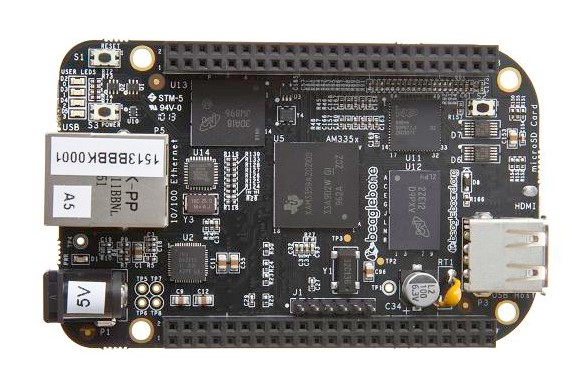
\includegraphics[angle=0,height=5cm]{images/BeagleBoneBlack.jpg}
\caption{Originaler BeagleBone Black}
\label{fig:BeagleBoneBlack}
\end{figure}


\section{Aufgabenstellung}
%Auftrag generell
Im Auftrag des Industriepartners Variosystems soll ein eigener, kostengünstiger und auf dem BeagleBone Black basierter Platinencomputer entwickelt werden. Dafür gilt es, ergänzend zu den eigentlichen Funktionen des BeagleBone Black, weitere Funktionen wie WLAN, Bluetooth Low-Energy, und GSM/GPRS zu integrieren. Zusätzlich soll ein TFT-Display mit einem kapazitivem Multi-Touch-Screen angeschlossen werden, welches von Variosystems zur Verfügung gestellt wird. Das Ganze soll dann als Einheit aufgebaut werden.

%Herstellbarkeit praktisch
Ziel der Arbeit ist es, dass Variosystems diesen Computer selber herstellen und nach Wunsch modifizieren kann. Die Produktionspläne sollen so aufbereitet werden, dass die benötigten PCBs bei einem PCB-Hersteller bestellt werden können. Die Bestückung der PCBs erfolgt dann bei Variosystems. Bei den Bauteilen ist ein besonderes Augenmerk auf die Lieferbarkeit zu werfen. Damit die Bauteile bestellt werden können, muss eine Bauteilliste, auch 'Bill of material' oder kurz BOM, erstellt werden. Diese Liste ist mit der Bestellnummer von üblichen Distributoren wie zum Beispiel Digi-Key oder Mouser zu ergänzen. Standartbauteile, wie etwa Widerstände, hat Variosystems auf Lager. Bei solchen Bauteilen muss auch die Artikelnummer von Variosystems für das entsprechende Bauteil in der BOM aufgeführt werden.

%Modularität, kritischer bereich, 
Die Hardware wie auch die Software sollen möglichst modular aufgebaut sein. Dies bedeutet für die Entwicklung der Hardware, dass alle Bauteile für eine bestimmte Funktion gruppiert und eindeutig erkennbar sein müssen. Ebenso sollen die Bauteile identifiziert werden, welche für die Lauffähigkeit des Computers unbedingt benötigt werden. Ein besonderes Augenmerk ist auf die Stellen zu werfen, bei denen die Leiterbahngeometrie relevant ist. Wie etwa bei der Hochgeschwindigkeitsschnittstelle zwischen Prozessor und RAM. Die Softwaretreiber sollen so geschrieben sein, dass die einzelnen Treiber ohne die anderen lauffähig sind. 

%Software
Zusätzlich zu den Treibern sollten auch Applikationen für die einzelnen Module entwickelt werden. Diese Applikationen sollen als Demonstration der Funktionen und als Vorlage für mögliche Anwendungen verwendet werden können.

	
	
	
	\chapter{Einleitung}


\section{Git-Repositories}
Dieses Dokument enthält die gesamte Dokumentation.
Zusätzlich wurden auf drei verschiedenen Git-Repositories entwickelt.

\textbf{Pseudo Sequencer}\\
Der \textit{Pseudo Sequencer} wurde am Anfang der Entwicklung geschrieben, um Zusammenhänge zu verstehen und das ganze Konzept logisch zu verstehen.
Er erhält Code, der C++ ähnelt, ist aber nicht lauffähig.
\begin{itemize}
\item \url{https://github.com/MarcelGehrig2/pseudoSequencer}
\end{itemize}

\textbf{TestApp}
Dieses Repository wurde synchron mit der EEROS-Repository mitentwickelt.
Wenn beim Sequenzer im EEROS-Repository eine neue Funktion eingebaut wurde, wurde sie vor dem Commit mit dieser Testapplikation getestet.
\begin{itemize}
\item \url{https://github.com/MarcelGehrig2/testAppVt1}
\end{itemize}

\textbf{EEROS-Repository}
Das EEROS-Repository ist ein Fork vom originalen EEROS-Repository (Hash: f4d8c8e32c138fdca5d1eb47d6e821c374c2cf07).
In diesem Repository wurde der Sequenzer entwickelt.
\begin{itemize}
\item \url{https://github.com/MarcelGehrig2/eeros-vt1}
\end{itemize}



\section{EEROS}
% kurze beschreibung von eeros
EEROS (Easy, Elegant, Reliable, Open and Safe) ist ein echtzeitfähiges, Open Source Software Framework, welches an der NTB entwickelt wurde und auch immer noch weiter entwickelt wird. 
Das Ziel von EEROS ist, möglichst zuverlässig und einfach in der Bedienung zu sein.
Da das Framework besonders auch in industriellen Robotern zum Einsatz kommen soll, ist besonders auch die Zuverlässigkeit der Software ein wichtiger Punkt.
Für die Software wird die objektorientierte Programmiersprache C++ verwendet. %TODO akronym für sw, besserer satz


EEROS kann in vier Hauptbereiche unterteilt werden.
\begin{enumerate}
\item Die HAL (Hardware Abstraction Layer), welche als Schnittstelle zur Hardware dient.
\item Das CS (\textit{ControlSystem}). Im CS wird die Regelung des Roboters aufgebaut.
In diesem System wird aber nicht nur die Regelung gerechnet, sondern auch Aufgaben wie die Berechnung der Vorwärts- und Inverskinematik werden hier erledigt.
\item Der Sequencer steuert den Ablauf des Roboters.
Hier werden sowohl Wegpunkte aufgelistet, wie auch das allgemeine Verhalten definiert. %TODO besserer satz
\item Im SS (\textit{SafetySystem}) werden sicherheitsrelevante Parameter überwacht. Das SS arbeitet unabhängig vom CS und vom Sequencer. Es löst ein Not-Aus aus, wenn der Roboter ausserhalb der zulässigen Parameter operiert. Ein möglicher Grund für ein Not-Aus wäre zum Beispiel, wenn sich der Roboterarm in einem Sicherheitsbereich zu schnell bewegt.
\end{enumerate}


%TODO bild eeros system




\section{Klarstellung der Benennungen}
% Mischung englisch deutsch
Die meisten Programmiersprachen werden in Englisch codiert.
Auch die offizielle Onlinedokumentation \cite{eerosOrg} von EEROS und die Benennung von Komponenten und Konzepten ist in Englisch.
In diesem Dokument wird an vielen Stellen bewusst darauf verzichtet, englische Bezeichnungen auf Deutsch zu übersetzen.
Dies kann zu Deutsch - Englischen Mischwörter führen.
Solche Mischwörter sind zwar nicht elegant, können aber besser für die Verständlichkeit sein und werden deshalb mit Absicht verwendet.
Auch einige Eigennamen, wie z.B. \textit{Sequencer} anstelle von \textit{Sequenzer}, werden in diesem Dokument nicht immer auf Deutsch übersetzt.

In dieser Arbeit wird oft von drei verschiedenen Kategorien von Entwicklern gesprochen.
Es wird zwischen EEROS-, Steuerungs- und Applikationsentwickler unterschieden.

Der \textbf{EEROS-Entwickler} hat vertiefte Kenntnisse der Programmiersprache C++ und vom EEROS Framework.
Seine Hauptaufgabe ist die Weiterentwicklung des Frameworks, welches vom Steuerungsentwickler verwendet wird.

Der \textbf{Steuerungsentwickler} hat ebenfalls gute C++ Kompetenzen und nutzt das Framework um eine Steuerung für einen Roboter zu entwickeln.
Dafür muss er seine Software speziell an den Roboter anpassen.
Er bereitet auch erste Sequenzen für den Applikationsentwickler vor.
Oft wird die Entwicklung der Steuerung und der Applikation von derselben Person übernommen.

Um den Ablauf des Roboters anzupassen kann der \textbf{Applikationsentwickler} bestehende Sequenzen einfach abändern.
Dazu werden nur grundlegende Programmierfähigkeiten benötigt.
Mit etwas erweiterten Kenntnissen kann er auch neue Sequenzen erstellen.



\section{Aufgabenstellung}
In der aktuellen Version von EEROS existiert bereits eine erste Version von einem Sequencer.
Dieser ist in seiner Funktionalität und Übersichtlichkeit aber stark eingeschränkt.
Oft musste auf Tricks zurückgegriffen werden, damit bestimmte Aufgaben mit dem bestehenden Sequencer gelöst werden konnten.
Um eine bestehende Sequenz anpassen zu können, auch wenn der Ablauf nur geringfügig geändert werden soll, ist schon viel Fachwissen notwendig.

In dieser Vertiefungsarbeit sollen diese beiden Probleme gelöst werden.
Es soll ein neuer Sequencer entwickelt werden, der flexibel für verschiedenste Arten von Robotern eingesetzt werden kann.
Die Sequenzen, welche den Ablauf des Roboters beschreiben, sollen dabei möglichst einfach und übersichtlich aufgebaut sein.
Dank des einfachen Aufbaus soll es auch für einen Applikationsentwickler möglich sein Sequenzen anzupassen und zu erstellen, auch wenn er keine vertieften Kenntnisse von C++ besitzt.

% vorgehen: requirement, konzept, ausarbeitung, implementierung
	\chapter{EEROS aktueller Stand}
\section{EEROS generell}
%TODO


\section{Aktuelle Implementierung des Sequencers}
Für EEROS besteht bereist ein rudimentärer \textit{Sequencer}.
Im folgenden Kapitel wird die bestehende Implementierung kurz erklärt.
In der Onlinedokumentation\footnote{http://wiki.eeros.org/eeros\_architecture/sequencer/start} wird noch vertiefter in die Details des bestehenden \textit{Sequencers} eingegangen, als in dieser Arbeit.


\subsection{Sequencer}
Die Grundlage bildet ein Sequencer-Objekt, das in einem Nicht-Realtime-Thread läuft.
In so einem \textit{Sequencer} können eine Serie von blockierenden \textit{Sequences} aufgerufen werden.
Wenn mehrere parallele \textit{Sequences} aufgerufen werden sollen, muss für jede \textit{Sequence} ein eigener \textit{Sequencer} erstellt werden.

\begin{figure}[!ht]
\centering
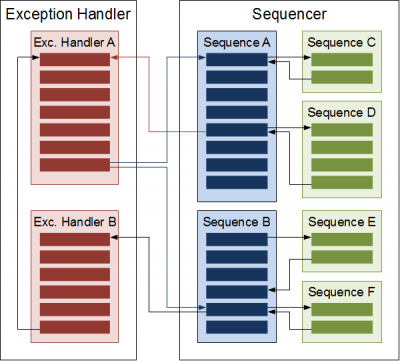
\includegraphics[angle=0,height=8cm]{images/SequencerBestehend.png}
\caption{Schematische Darstellung des bestehenden Sequencers \protect\footnote{http://wiki.eeros.org/eeros\_architecture/sequencer/start}}
\label{sequencerBestehend}
\end{figure}


\subsection{Sequence}
Eine \textit{Sequence} führt als erstes eine benutzerdefinierte Initialisierungsfunktion aus.
Als nächstes wird eine \textit{preCondition} überprüft.
Fehlt die Überprüfung fehl, wird die \textit{Sequence} abgebrochen.
Bei einem positiven Ergebnis wird der Hauptteil, eine Abfolge von definierten \textit{Steps} ausgeführt.
Dem letzten \textit{Step} folgt noch eine Überprüfung einer \textit{postCondition}.
Läuft der \textit{Sequencer} im \textit{stepping-mode}, wird die \textit{Sequence} bei jeden \textit{yield()} pausiert und wird erst fortgeführt, wenn der Befehl dazu gegeben wird.\footnote{http://wiki.eeros.org/eeros\_architecture/sequencer/start}

\begin{lstlisting}
init();
yield();

if(!checkPreCondition()) 
  return SequenceResult<void>(result::preConditionFailure);
yield();

run();
yield();

if(!checkPostCondition())
  return SequenceResult<void>(result::postConditionFailure);
yield();

exit();
return SequenceResult<void>(result::success);
\end{lstlisting}


\subsection{Step}
Ein \textit{Step} ist eine vom \textit{Steuerungsentwickler} festgelegte Einheit, die von einem \textit{yield()} Befehl unterteilt wird.
\textit{Steps} können im \textit{stepping-mode} einzeln abgearbeitet werden.


\subsection{Sub-Sequence}
\textit{Subsequences} sind sehr ähnlich wie normale \textit{Sequenzen}.
Sie können verwendet werden, wenn ein ähnlicher Ablauf mehrmals wiederholt werden soll.
Durch eine Übergabe von Parameter an eine solche \textit{Subsequence} kann sie sehr flexibel gestaltet werden.
Wenn die \textit{Subsequence} parallel, also nicht-blockierend, aufgerufen werden soll, muss sie einem neuen Sequencer übergeben werden.

\begin{lstlisting}
class SequenceB : public Sequence<> {
public:
  SequenceB(std::string name, Sequencer* seq, Robot& r) : Sequence<void,double>(name, seq), robot(r){ }
 
  void run() {
    robot.moveZ(5);
    sleep(3);
    yield();
    robot.moveZ(0);
  }
 
private: 
  Robot& robot;
};
\end{lstlisting}


\subsection{Error-Handler}
Der \textit{Error-Handler} wird in der Onlinedokumentation zwar erwähnt, im Sourcecode von EEROS sind aber keine Spuren von der Implementierung zu finden.
Der Dokumentation zu folge soll er \textit{Exceptions} behandeln.
Je nach \textit{Exception} soll er flexibel reagieren, um Probleme zu beheben.



%\section{Fallbeispiel Parallel Scara}
%
%\begin{figure}[!ht]
%\centering
%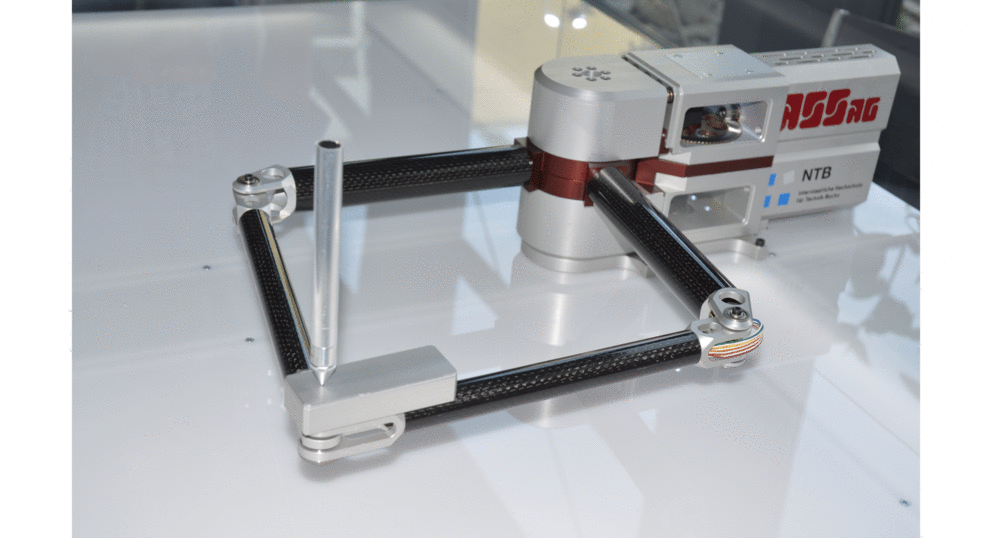
\includegraphics[angle=0,height=8cm]{images/ParallelScara.png}
%\caption{Der Parallel Scara Roboter \protect\footnote{http://www.ntb.ch/projekt/parallel-scara/}}
%\label{parallelScara}
%\end{figure}
%
%Der Parallel Scara ist ein Roboter, dessen Hardware und auch Software an der NTB entwickelt wurde.
%Die Steuerung ist mit EEROS und dem bestehenden \textit{Sequencer} aufgebaut.
%Im folgenden Kapitel wird der Quellcode der Steuerung analyisiert um herauszufinden, welche Aspekte des bestehenden \textit{Sequencers} brauchbar sind, und wo er noch Lücken aufweist.
%
%
%\subsection{asdf}



\section{Fallbeispiel 'EEDURO Delta Roboter'}

%\begin{figure}[!ht]
%\centering
%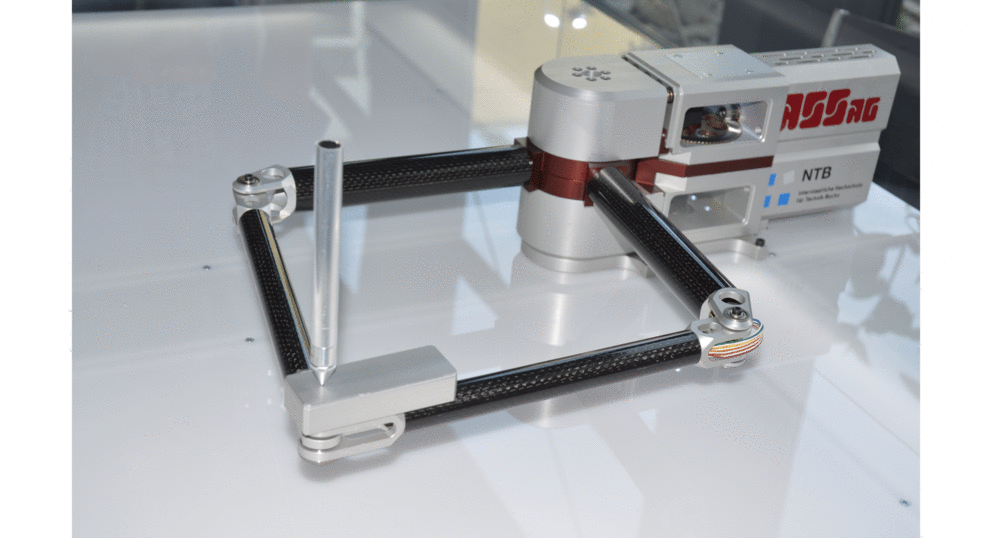
\includegraphics[angle=0,height=8cm]{images/ParallelScara.png}
%\caption{Der Parallel Scara Roboter \protect\footnote{http://www.ntb.ch/projekt/parallel-scara/}}
%\label{parallelScara}
%\end{figure}

Der \textit{EEDURO Delta Roboter} ist ein Roboter, dessen Hardware und auch Software an der NTB entwickelt wurde.
Die Steuerung ist mit EEROS und dem bestehenden \textit{Sequencer} aufgebaut.
Im folgenden Kapitel wird der Quellcode der Steuerung analyisiert um herauszufinden, welche Aspekte des bestehenden \textit{Sequencers} brauchbar sind, und wo er noch Lücken aufweist.

Der Quellcode der Steuerungssoftware ist auf folgendem Git-Repository zu finden: \\
\textit{https://github.com/ClaudiaVisentin/eeduro-platform }

%Die Software wurde vom Stand 10.10.2016 mit folgendem Hashverwendet: \\ \textit{a25bcfa752516723f067f5a5166e8f09e60fc6e8}
Die Software wurde vom Stand 10.10.2016 mit dem Hash \textit{\seqsplit{a25bcfa752516723f067f5a5166e8f09e60fc6e8}} verwendet.


\subsection{asdf}

	\chapter{Anforderungen an den Sequencer}
%TODO wie wurden ziele ausgearbeitet
\section{Formulierung der Anforderungen}
Im folgenden Kapitel werden die Anforderungen an den \textit{Sequencer} beschrieben.
Die Kapitel \textit{Ziele}, \textit{Nicht Ziele} und \textit{Test Cases} beschreiben die Anforderungen auf verschiedene Arten.
In \textit{Ziele} und \textit{Nicht Ziele} wird abstrakt beschrieben, welche Funktionen der neue \textit{Sequencer} beinhalten, beziehungsweise nicht beinhalten muss.
Im Kapitel \textit{Test Cases} werden verschiedene Fälle beschrieben die mit dem neuen \textit{Sequencer} möglichst elegant gelöst werden sollen.



\section{Ziele}
\subsection{Einfaches Interface für den Applikationsentwickler}
Mit dem bestehenden \textit{Sequencer} sind vertiefte Programmierkenntnisse notwendig, um eine Sequenz zu erstellen, oder abzuändern.
Sequenzen sind nicht intuitiv verständlich.
Es werden Kenntnisse vom \textit{Control System} und dem \textit{Safety System} benötigt, um einen neuen Ablauf für den Roboter schreiben zu können. %TODO Satz
Zurzeit werden Sequenzen von den Steuerungsentwickler geschrieben.

Wenn der Roboter fertig entwickelt worden ist, soll er an einen Kunden übergeben werden können.
Der Kunde, oder der Betreiber des Roboters, soll dann Änderungen im Ablauf des \textit{Sequencers} vornehmen können, ohne dass er vertiefte Kenntnisse von der Programmiersprache C++ oder von der inneren Funktionsweise des Roboters haben muss.
Dafür ist es notwendig, dass der Steuerungsentwickler den Roboter so abstrahiert, dass die Sequenzen aus logischen und verständlichen Schritten bestehen.


\subsection{Flexibel einsetzbar für verschiedenste Arten von Roboter}
Auch wenn die Sequenzen möglichst einfach aufgebaut werden sollen, muss der \textit{Steuerungsentwickler} für alle möglichen Kategorien von Robotern Sequenzen bauen können.
Verschiedene Arten von Roboter haben verschiedene Anforderungen.
Das \textit{Control System} von einem Roboterarm mit sechs Freiheitsgraden unterscheidet sich stark von einer Fertigungsstrassen mit mehreren Förderbändern.
Trotz diesen Unterschieden soll es möglich sein, für beide Kategorien von Robotern sinnvolle Sequenzen zu erstellen.
Das bedeutet, dass der \textit{Steuerungsentwickler} möglichst viele Freiheiten beibehält, ohne dass er durch das \textit{Framework} unnötig begrenzt wird.
%TODO ss missbraucht


\subsection{Parallele und blockierende Sequenzen}
Wie bereits im bestehenden Sequenzer verwirklicht wurde, sollen Sequenzen blockierend und nicht-blockierend aufgerufen werden können.
Diese Funktion von blockierenden und parallel ausgeführten Sequenzen soll auch im neuen \textit{Sequencer} beibehalten werden.
 

\subsection{Exception Handling}
Eine \textit{Exception} ist ein Ereignis, dass nicht immer auftritt, aber auftreten kann.
Zu solchen \textit{Exception}, oder Ausnahmen, gehören zum Beispiel:
\begin{enumerate}
\item Ein blockiertes Förderband
\item Ein Timeout
\item Der Roboter soll ein Paket abholen, dass nicht vorhanden ist
\end{enumerate}
Solche Ausnahmen sollen im \textit{Sequencer} erkennt werden können und flexibel darauf reagiert werden können.
Eine solche Reaktion könnte eine spezielle Sequenz sein, die versucht, eine solche Ausnahme zu behandeln.
Alternativ soll aber auch die aktuelle Sequenz abgebrochen, oder neu gestartet werden können.


\subsection{Zugriff auf Control System}
Der aktuelle \textit{Sequencer} nutzt ein Pointer auf das \textit{Control System} um Blöcke direkt auslesen und schreiben zu können.
Wenn das \textit{Control System} betrachtet wird, kann nicht festgestellt werden, welche Blöcke vom \textit{Sequencer} ausgelesen oder geschrieben werden.
Ein klares Interface zum \textit{Sequencer} wäre wünschenswert, um das \textit{Control System} übersichtlicher zu machen.


\subsection{Safety System entlasten}
Eine Analyse von bestehenden Implementationen des alten \textit{Sequencers} hat gezeigt, dass das \textit{Safety System} viele Aufgaben übernimmt, welche besser vom \textit{Sequencer} übernommen werden sollten.
Das \textit{Safety System} sollte möglichst nur eingesetzt werden, um das System zu überwachen.
Alle anderen Aufgaben sollen vom \textit{Sequencer} oder vom \textit{Control System} übernommen werden.



\section{Nicht Ziele}
\subsection{Echtzeit}
Das \textit{Control System} und das \textit{Safety System} laufen beide in einem Echtzeit-Task.
Der \textit{Sequencer} soll aber bewusst nur mit normaler Priorität laufen und besitzt keine Echtzeit Fähigkeit.

Da der \textit{Sequencer} keine Regelung berechnet, benötigt er keine Echtzeit Fähigkeit.
Eine niedrigere Priorität als das \textit{Control System} und das \textit{Safety System} ist notwendig, dass die beiden Systeme nicht vom \textit{Sequencer} beeinträchtigt werden.


\subsection{Pfadplanung}
Die Pfadplanung ist nicht Teil des \textit{Sequencers}, da sie den Rahmen dieser Arbeit sprengen würde.



\section{Test Cases}
\subsection{Einleitung}
Die Testfälle sind so aufgebaut, dass sie möglichst einfach und elementar sind.
Jeder \textit{Test Case} beschreibt eine andere Anforderung oder Spezialfall an den \textit{Sequencer}.
Alle in der Realität vorkommenden Situation sollte durch einen, oder einer Kombination von mehreren, \textit{Test Cases} beschrieben werden können.

Eine Ausnahme dazu bildet \textit{Test Case 8}.
In diesem Testfall wurden möglichst viele verschiedene Situationen vereint.

Mit dem \textit{Sequencer} sollen alle Testfälle sauber und elegant umgesetzt werden werden können.


\subsection{Test Case 1: Achse einfach}
\textbf{System}
\begin{itemize}
\item Eine Achse die sich nach links und rechts bewegen kann
\item An beiden Enden befindet sich ein Endschalter
\item Ein Taster \textit{Taster links}, der die Achse nach links laufen lässt
\item Ein Taster \textit{Taster rechts}, der die Achse nach rechts laufen lässt
\end{itemize}

\textbf{Aufgabe}
\begin{itemize}
\item Solange \textit{Taster links} gedrückt bleibt, fährt die Achse nach links
\item Solange \textit{Taster rechts} gedrückt bleibt, fährt die Achse nach rechts
\item Die Achse hält an, wenn einer der beiden Endschalter erreicht wird
\end{itemize}

\textbf{Herausforderungen}
\begin{itemize}
\item Der \textit{Sequencer} muss die Eingänge \textit{Taster links}, \textit{Taster rechts} und die beiden Endschalter permanent überwachen und auf eine Änderung reagieren.
\end{itemize}


\subsection{Test Case 2: EEDURO Delta Roboter Maus}
\textbf{System}
\begin{itemize}
\item EEDURO Delta Roboter mit Maus
\end{itemize}

\textbf{Aufgabe}
\begin{itemize}
\item Während dem Idle Zustand wird auf einen Input von der Maus gewartet
\item Wenn sich die Maus für fünf Sekunden nicht bewegt, wird eine blockierende \textit{Autor-Sort Sequenz} gestartet
\item Bewegt sich die Maus innerhalb von fünf Sekunden, dann bewegen sich die Achsen entsprechend der Mausbewegung und der 5-Sekunden-Timer wird neu gestartet
\end{itemize}

\textbf{Herausforderungen}
\begin{itemize}
\item Timeout
\item Blockierende Sequenz
\end{itemize}


\subsection{Test Case 3: Rendezvous}
\textbf{System}
\begin{itemize}
\item Greifer Zubringer
\item Greifer Abholer
\item Paket: Gegenstand, der übergeben wird
\item Förderband Zubringer: Hält ständig ein neues Paket bereit für \textit{Greifer Zubringer}
\item Förderband Abholer: Transportiert ständig alle Pakete weg, welche vom \textit{Greifer Abholer} abgelegt werden
\end{itemize}

\textbf{Ablauf (Siehe Abbildung \ref{Testcase03Picture}})
\begin{enumerate}
\item Der \textit{Greifer Zubringer} holt ein neues Paket vom \textit{Förderband Zubringer}
\item Der \textit{Greifer Zubringer} bringt das Paket in Rendezvous-Position
\item Der \textit{Greifer Abholer} übernimmt das Paket vom \textit{Greifer Zubringer} 
\item Der \textit{Greifer Abholer} legt das Paket auf das \textit{Förderband Abholer}
\item Die Sequenz beginnt wieder von Anfang an
\end{enumerate}

%\begin{figure}[!ht]
\begin{figure}[]
\centering
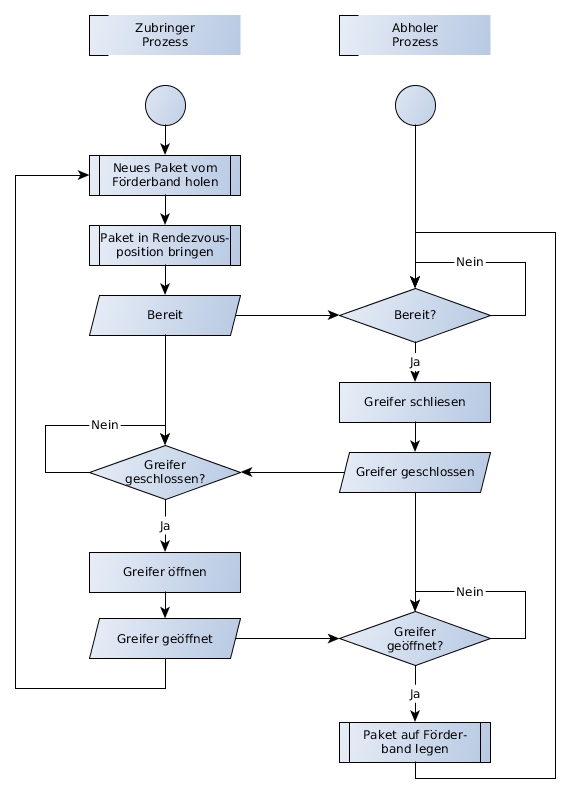
\includegraphics[angle=0,height=10cm]{images/Testcase03.png}
\caption{\textit{Test Case 3}: Ablaufdiagramm vom}
\label{Testcase03Picture}
\end{figure}

\textbf{Herausforderungen}
\begin{itemize}
\item Synchronisation von zwei parallellaufenden Sequenzen
\item Kommunikation zwischen zwei Sequenzen
\end{itemize}


\subsection{Test Case 4: Sequenz pausieren}
\textbf{System}
\begin{itemize}
\item Roboterarm
\item Ein Taster \textit{Taster Pause}, der die Sequenz pausiert
\end{itemize}

\textbf{Ablauf}
\begin{itemize}
\item Der Roboterarm führt eine sich wiederholende Sequenz endlos aus
\item Wird \textit{Taster Pause} gedrückt, pausiert die Sequenz
\item Wird \textit{Taster Pause} erneut gedrückt, wird die Sequenz fortgeführt
\end{itemize}

\textbf{Herausforderungen}
\begin{itemize}
\item Jede Sequenz muss jederzeit pausiert werden können
\item Der Taster gibt nur einen Impuls, nicht eine bleibende Pegeländerung an einem Eingang
\item Timeouts müssen pausiert werden
\end{itemize}


\subsection{Test Case 5: Zwei Roboterarme}
\textbf{System}
\begin{itemize}
\item Roboterarm A
\item Roboterarm B
\item Ein Taster \textit{Taster Pause}, der beide Sequenzen pausiert
\end{itemize}

\textbf{Ablauf}
\begin{itemize}
\item Beide Roboterarme führen sich wiederholende Sequenz endlos aus
\item Wird \textit{Taster Pause} gedrückt, pausieren beide Sequenzen
\end{itemize}

\textbf{Herausforderungen}
\begin{itemize}
\item Zwei parallellaufende Sequenzen müssen mit einem Taster pausiert werden können
\end{itemize}


\subsection{Test Case 6: Prellender Taster}
\textbf{System}
\begin{itemize}
\item Ein prellender Taster \textit{Taster A}
\end{itemize}

\textbf{Aufgabe}
\begin{itemize}
\item Ein prellender Taster soll sauber eingelesen werden
\end{itemize}

\textbf{Herausforderungen}
\begin{itemize}
\item Der Taster muss entprellt werden
\item Mehrmaliges drücken soll sauber registriert werden, auch wenn der Taster in schneller Abfolge gedrückt wird
\end{itemize}

\begin{figure}[]
\centering
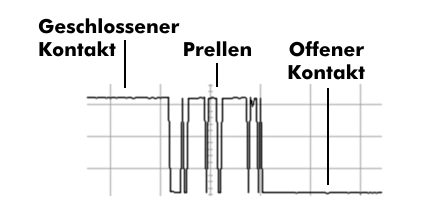
\includegraphics[angle=0]{images/Testcase06.png}
\caption{\textit{Test Case 6}: Signalverlauf bei einem prellenden Schalter}
\label{Testcase06Picture}
\end{figure}


\subsection{Test Case 7: Menü}
\label{Testcase07}
\textbf{System}
\begin{itemize}
\item Ein beliebige Anzahl Taster \textit{Taster A}, \textit{Taster B}, \textit{Taster C}, ....
\end{itemize}

\textbf{Aufgabe}
\begin{itemize}
\item Wenn sich das System in einem \textit{Idle} Zustand befindet, soll jeder Taster eine andere Sequenz starten
\end{itemize}

\textbf{Herausforderungen}
\begin{itemize}
\item Dieses \textit{Menü} lässt sich nicht im klassischen Sinne als eine Sequenz, also eine Abfolge von Schritten, beschrieben werden. Trotzdem soll eine einfache Implementierung im \textit{Sequencer} möglich sein
\end{itemize}


\subsection{Test Case 8: Detailliertes Rendezvous}
Dieser \textit{Test Case} basiert auf auf dem \textit{Test Case 3}, ist aber detaillierter ausgearbeitet.
Im Anhang \ref{sec:anhang_test_case_8} ist das Ablaufdiagramm der Hauptsequenz \textit{Sequenz Rendezvous} und der blockierenden Subsequenz \textit{Sequenz PickUp} angehängt.
Das Ziel von diesem \textit{Test Case} war es nicht einen realistischen Fall abzubilden.
Viel mehr dient er dazu, möglichst viele Fälle und Situationen abzubilden, die in einer Sequenz vorkommen können.

%TODO grundlage für diskus

Das Ablaufdiagramm besteht aus folgenden Blöcken:
\begin{itemize}
\item Rechtecke: einzelne Steps
\item Rechtecke mit doppelten, vertikalen Linien: Blockierende Subsequenzen
\item Blaue Rauten: Entscheidungen
\item Grüne Rauten: Blockierungen, bis Entscheidung wahr wird
\item Parallelogramm: Statusvariable wird geändert
\item Lange senkrechte Rechtecke: Bedingung, welche über längere Zeit überwacht wird
\end{itemize}




	
	\chapter{Dokumentation für Steuerungsentwickler}
Dieses Kapitel ermöglicht einen leichten Einstig in den neuen Sequencer.
Es deckt aber nicht vollständig alle Details von allen Funktionen des Sequencer ab.
Eine detailliertere Beschreibung des Sequencers und von dessen Funktionen findet sich im Kapitel \ref{sequencerAufbau}.


\section{Den Sequencer erstellen}
Im Hauptprogramm der Applikation muss der Sequenzer erst erstellt werden.
Die Hauptsequenz, in diesem Beispiel \textit{mainSequence} genannt, wird in einem Thread gestartet, sobald sie dem Sequencer hinzugefügt wird.
Alle anderen Sequenzen werden von der Hauptsequenz aus gestartet.

\textit{main.cpp:}\
\begin{lstlisting}
#include "sequences/MainSequence.hpp"

eeros::sequencer::Sequencer S;
MainSequence mainSequence(S, &controlSystem, "mainSequence");
S.addMainSequence(&mainSequence);

executor.run();
mainSequence.join();	//The application only stops, when the mainSequence is finished
\end{lstlisting}


\section{Benutzerdefinierte Sequenz}
\subsection{Eigenschaften von Sequenzen}
Sequenzen werden standardmässig nicht-blockierend gestartet.
Es besteht aber auch die Möglichkeit, Sequenzen blockierend zu starten.


\subsection{Vorteile von benutzerdefinierten Sequenzen}



\subsection{Beispiel für eine mainSequence}

\textit{MainSequence.hpp:}\
\begin{lstlisting}
#include "SequenceA.hpp"
#include "SequenceB.hpp"
#include "SequenceExceptionA.hpp"

namespace testappsequencer {

	class TestAppCS;
	
	class MainSequence : public eeros::sequencer::Sequence {
	public:
		MainSequence(Sequencer& S, TestAppCS* CS, std::__cxx11::string name);

		int action();
		
		SequenceA seqA1;
		SequenceB seqB1; 
		SequenceB seqB2; 
		SequenceB seqB3;
		
		SequenceExceptionA seqEA1;
		
		TestAppCS* CS;
	};
};
\end{lstlisting}

Jede Sequenz muss von der Klasse \textit{eeros::sequencer::Sequence} abgeleitet werden.

\textbf{Zeile 7} und \textbf{Zeile 22} sind notwendig, um einen Pointer auf das \textit{ControlSystem} zu erhalten.
Dafür muss zusätzlich der \textit{Constructor} angepasst werden.

\textit{int action();} ist die wichtigste Methode der Sequenz.
Sie beinhaltet den Ablauf der Sequenz.

\textbf{Zeile 15} bis \textbf{Zeile 20} beschreiben benutzerdefiniert Sequenzen, die von der Hauptsequenz aus gestartet werden.


\textit{MainSequence.cpp:}\
\begin{lstlisting}
#include "MainSequence.hpp"

using namespace testappsequencer;
using namespace eeros;
using namespace eeros::sequencer;


MainSequence::MainSequence(Sequencer& S, TestAppCS* CS, std::__cxx11::string name) :
Sequence(S, name), CS(CS),

seqA1(S, CS, this, "seqA1"),
seqB1(S, CS, this, "seqB1"),
seqB2(S, CS, this, "seqB2"),
seqB3(S, CS, this, "seqB3"),
seqEA1(S, CS, this, "seqEA1")		//Exception Sequence
{
	setIsNonBlocking();
	
	seqA1.setTimeoutTime(5.1);
	seqA1.setTimeoutExceptionSequence(&seqEA1);
	seqA1.setTimeoutBehavior(restartOwner);
	
	seqA1.setIsBlocking();
}

int MainSequence::action()
{
	seqB1();
	seqB2();
	seqA1(10, 3);
	seqB3();
	
	seqB1.join();
	seqB2.join();
	seqB3.join();
	
	log.info() << "MainSequence ended";
}
\end{lstlisting}

In \textbf{Zeile 9} wird die Basis-Sequenz und der Pointer für das \textit{ControlSystem} initialisiert.
Zusätzlich müssen auch alle Sequenzen, die in dieser Sequenz genutzt werden, initialisiert werden.

\textbf{Zeile 17} definiert diese Sequenz als nicht-blockierend.
Die Hauptsequenz von einer Applikation muss immer nicht-blockierend sein.
Andere Sequenzen können blockierend sein.

Die \textbf{Zeile 19} aktiviert für die Sequenz \textit{seqA1} den Timeout und setzt die Zeit auf 5.1 Sekunden.
Wenn \textit{seqA1} nach 5.1 Sekunden Laufzeit noch nicht fertig abgearbeitet wurde, wird \textit{seqEA1} ausgeführt.
Nachdem die Exception-Sequenz \textit{seqEA1} beendet wurde, wird \textit{seqA1} neu gestartet, da dieses Verhalten in \textbf{Zeile 21} definiert wurde.

Durch den Befehl in \textbf{Zeile 23} wird \textit{seqA1}, unabhängig vom vordefinierten Standard von \textit{SequenceA}, blockierend ausgeführt.

In der Methode \textit{action()} wird der eigentliche Ablauf von der Sequenz definiert.
Als erstes wird \textit{seqB1} gestartet.
Da sie, und auch \textit{seqB2}, nicht-blockierend sind, wird sofort auch \textit{seqB2} und \textit{seqA1} gestartet.
Weil \textit{seqA1} den weiteren Ablauf blockiert, bis sie fertig gestellt wurde, wird \textit{seqB3} erst ausgeführt, wenn \textit{seqA1} beendet wurde.

Mit den \textit{join()}-Befehlen kann sichergestellt werden, dass die Hauptsequenz erst dann beendet wird, wenn die entsprechenden, parallel laufenden Sequenzen fertig abgearbeitet wurden.


\subsection{Beispiel für eine benutzerdefinierte Sequenz 'SequenceA'}

\textit{SequenceA.hpp:}\
\begin{lstlisting}
#include "SequenceExceptionA.hpp"

namespace testappsequencer {
	
	using namespace eeros::sequencer;
	
	class TestAppCS;
	
	class SequenceA : public Sequence {
	public:
		SequenceA(Sequencer& S, TestAppCS* CS, BaseSequence* caller, std::__cxx11::string name);
		
		int operator()(int a, int b);
		//int operator()(std::string str);
		//int operator()();
		int action();
		
		SequenceExceptionA seqEA2;
		
		TestAppCS* CS;
		int posA;
		int posB;
	};
};
\end{lstlisting}

Der Aufbau von dieser Sequenz ähnelt stark dem Aufbau von der Hauptsequenz.
Der einzige Unterschied ist die Methode \textit{int operator()(int a, int b);}.
Diese Methode wird aufgerufen, bevor die Sequenz gestartet wird und kann genutzt werden, um Parameter zu übergeben.
Je nach Bedarf können die Typen und Anzahl der Parameter frei gewählt werden, oder mit \textit{int operator()();} ganz weggelassen werden.


\textit{SequenceA.cpp:}\
\begin{lstlisting}
#include "SequenceA.hpp"
#include "../steps/StepA.hpp"

using namespace testappsequencer;


SequenceA::SequenceA(Sequencer& S, TestAppCS* CS, BaseSequence* caller, std::__cxx11::string name)
: Sequence(S, caller, name), CS(CS),

seqEA2(S, CS, this, "seqEA2Step")
{
	setIsBlocking();
}


int SequenceA::operator()(int a, int b)
{
	posA = a;
	posB = b;
	return Sequence::start();	//this code is mandatory for every derived Step- and Sequence-Class
}


int SequenceA::action()
{
	//initialisation of the step 'goTo'
	GoTo goTo = StepA(S, CS, this);
	sA.setTimeoutTime(5);
 	sA.setTimeoutBehavior(abortOwner);
	sA.setTimeoutExceptionSequence(&seqEA2);
	
	//start of the sequence
	goTo(0);
	goTo(posA);
	goTo(posB);
}

\end{lstlisting}

Mit dem Befehl \textit{setIsBlocking()} im Konstruktor werden standardmässig alle Sequenzen von der Klasse \textit{SequenceA} blockierend ausgeführt.
Der Befehl \textit{seqA1.setIsBlocking();} aus \textit{MainSequence.cpp} wäre somit gar nicht notwendig.

Es ist zwingen notwendig, dass die Methode \textit{operator()} implementiert wird.
Ebenfalls erforderlich ist, dass der letzte Befehl von dieser Methode \textit{return Sequence::start();}  lautet.
Wenn der Sequenz Parameter übergeben werden, dann können hier die Variablen gespeichert werden.

Am Anfang der \textit{action()}-Methode wird ein neuer \textit{Step} initialisiert.
\textit{Steps} verhalten sich sehr ähnlich wie Sequenzen.
Sie können aber nur blockierend aufgerufen werden.
Da \textit{Steps} keinen eigenen Thread starten, brauchen sie weniger Ressourcen und können einfach mehrmals hintereinander aufgerufen werden.



\subsection{Beispiel für einen benutzerdefinierten Step 'GoTo'}

\textit{GoTo.hpp:}\
\begin{lstlisting}
#include <eeros/sequencer/Step.hpp>

namespace testappsequencer {
	
	using namespace eeros::sequencer;
	
	class  TestAppCS;
	
	class GoTo : public Step {
	public:
		GoTo(Sequencer& S, TestAppCS* CS, BaseSequence* caller);
		
		int operator()(int a, int b);
		int action();
		bool checkExitCondition();
		
		TestAppCS* CS;
	};

	
	
};
\end{lstlisting}
	%\include{DokumentationFuerApplikationsentwickler}
	\chapter{Aufbau des Sequencers}


\section{Caller Stack}
Das unterste (älteste) Element ist die ID-Nummer der Hauptsequenz.
Als nächstes folgt 
 %innerer Aufbau
	%\chapter{Test des Sequencer}


\section{section}
	\chapter{Ergebnis, Fazit und Ausblick}
\section{Ergebnis}
Der entwickelte Sequenzer löst viele Probleme des alten Sequenzer.
Es ist nun möglich Sequenzen so zu bauen, dass sie auch für Nicht-Experten einfach verständlich sind.

Die Klasse \textit{Condition} erlaubt es nun, komplexe zusammenhängende Zustände in einer Klasse zu Abstrahieren.
Der \textit{Steuerungsentwickler} kann eine benutzerdefinierte Klasse ableiten, die der \textit{Applikationsentwickler} nutzen kann, ohne dass er die implementierte Funktionalität verstehen muss.
Der selbe Vorteil besteht auch für \textit{Sequenzen} und \textit{Steps}.

Mit den neuen \textit{Monitore} existiert eine einfache Möglichkeit, bestimmte Zustände permanent und automatisch zu überwachen.
Die \textit{Monitore} können zusammen mit den \textit{Conditions} als Exception-Handler verwendet werden.

Eine Synchronisation und Datenaustausch zwischen mehreren parallel laufenden Sequenzen ist einfach möglich, da jetzt nur noch der Namen der gesuchten Sequenz bekannt sein muss, um einen Pointer auf die Sequenz zu erhalten.


\section{Fazit}	%subjektiv
Ich habe sehr viel Zeit für den Pseudo-Sequenzer aufgewendet.
Der Plan, den Sequenzer mit Hilfe des Pseudo-Sequnzers genau durchzuplanen und ihn dann in das Framework zu integrieren, ist aber nicht aufgegangen.
Bei der Integration ins EEROS habe ich gemerkt, dass viele Konzepte nicht so funktionierten, wie ich es geplant hatte.
Einige Teile konnte ich mit aufwändig in kleinen Schritten integrieren, andere Teile musste ich verwerfen und neu durchdenken, weil sie nicht möglich waren.

Die vielen unvorhergesehenen Komplikationen haben meinen Zeitplan durcheinander gebracht.
Aus diesem Grund konnte ich die Software nicht ausgiebig testen.

In dieser Arbeit habe ich nicht nur vieles neues Wissen bezüglich der Programmiersprache C++ aneignen, ich habe auch eine Lektion in Software-Management gelernt.
Für Software eignet sich der Ansatz, erst alles durchplanen, dann alles integrieren und am Schluss die komplette Software durchtesten, nicht gut.
In meinem nächsten Software-Projekt werde ich viel mehr auf kleine, aber dafür viele Iterationen planen-implementieren-testen setzen.
Diese Strategie habe ich bei dieser Arbeit leider erst am Schluss eingesetzt.
Besonders auf das Testen werde ich bei der nächsten Arbeit grösseren Wert legen.


\section{Ausblick}
Der neue Sequenzer bildet eine gute Grundlage für einfach verständliche Abläufe mit sehr hoher Flexibilität.
Allerdings wurde er noch nicht ausgiebig getestet, so dass keine Aussage über die Zuverlässigkeit gemacht werden kann.

Des weiteren gibt es noch einige offene Punkte:
\begin{itemize}
\item Genau überprüfen, ob alle Ziele erreicht wurden.
\item Race-Condition. Zum Beispiel wenn mehrere parallel laufende Sequenzen auf das \textit{SafetySystem} oder das \textit{ControlSystem} zugreifen wollen.
\item Geregelter Zugriff auf das \textit{ControlSystem}. Evt. wird von einer Sequenz exklusiven Zugriff auf Teile des \textit{ControlSystem} verlangt, so dass sie nicht von einer anderen Sequenz gestört wird.
\item Onlinedokumentation auf der EEROS-Homepage nachführen.
\end{itemize}

	
	
	
%%	\glossary{name={eCAD},description={Electronic Computer-Aided Design: Computerprogramm zum Entwerfen von elektrischen Layouts und PCB}}

\glossary{name={PCB},description={Printed Circuit Board: Elektronische Platine, auf welcher die elektronischen Bauteile aufgelötet werden. Wird auch Platine genannt.}}

\glossary{name={BBB},description={BeagleBone Black: Kostengünstiger Einplatinen-Computer von Texas Instruments}}

\glossary{name={BBB-Derivat},description={BeagleBone-Derivat: Das Produkt, das in dieser Bachelorarbeit in Zusammenarbeit mit Variosystems hergestellt wurde. Es hat den selben Funktionsumfang wie der BBB}}

\glossary{name={BeagleBone Black},description={Siehe BBB}}

\glossary{name={PHY},description={PHYsical Layer: Spezieller integrierter Schaltkreis der die modulierten analogen Daten des LAN-Anschlusses in digitale Daten wandelt und umgekehrt. Dieses Bauteil wird zusammen mit einer RJ45-Buchse und einem MAC für eine Ethernet-Schnittstelle benötigt}}

\glossary{name={MAC},description={Media Access Control: Dieser Controller wird zusammen mit einer RJ45-Buchse und einem PHY für eine Ethernet-Schnittstelle benötigt }}

\glossary{name={HDMI},description={High Definition Multimedia Interface: Eine Schnittstelle für die volldigitale Übertragung von Audio- und Videodaten}}

\glossary{name={eMMC},description={Embedded Multimedia Card: Massenspeicher mit Flashspeicher, MMC-Interface und Controller. Ersetzt im BBB die Festplatte}}

\glossary{name={awk},description={Skriptsprache zur Bearbeitung und Auswertung strukturierter Textdaten, beispielsweise CSV-Dateien}}

\glossary{name={Designator},description={Eindeutige Bezeichnung aus einem Buchstaben und einer Zahl für ein elektrisches Bauteil in einem Schema oder PCB-Layout}}

\glossary{name={Cape},description={Erweiterung speziell für den BBB}}

\glossary{name={WLAN},description={Kabelloser Standard für LAN}}

\glossary{name={BLE},description={Bluetooth Low Energy: Standard für eine Funktechnik, die mit sehr geringen Stromverbrauch Geräte in einer Umgebung von 10 Meter vernetzen kann}}

\glossary{name={LCD},description={Liquid Cristal Display: Flachbildschirm}}

\glossary{name={SDIO},description={Secure Digital Input Output: Vielseitiger Datenbus, welcher unter Anderem für SD-Karten verwendet wird}}

\glossary{name={I$^2$C},description={Inter-Integrated Circuit: serieller Datenbus, welcher für die Kommunikation zwischen Bauteilen auf einem PCB verwendet wird}}

\glossary{name={EEPROM},description={Electrically Erasable Programmable Read-Only Memory: nichtflüchtiger, elektronischer Speicher für kleine Datenmengen}}

\glossary{name={RAM},description={Random-Access Memory: wird von Prozessoren als Arbeitsspeicher benötigt}}

\glossary{name={Python},description={Universelle Programmiersprache}}

\glossary{name={SMT},description={Surface Mounted Technology: Oberflächenmontage. Die elektrischen Bauteile werden nur auf der Oberfläche des PCB gelötet}}

\glossary{name={THT},description={Through Hole Technology: Durchsteckmontage. Die Bauelemente haben Drähte als Anschluss, die durch das PCB gesteckt werden}}

\glossary{name={McASP},description={Multichannel Audio Serial Port: Datenbus für Audiodaten}}

\glossary{name={Footprint},description={Die Umrisse von Lötflächen von elektrischen Bauelementen auf einer Leiterplatte}}





\glossary{name={USB},description={Universal Serial Bus: Serielles Bussystem zur Verbindung eines Computers mit externen Geräten}}

\glossary{name={LAN},description={Local Area Network: Netzwerk mit einer Ausdehnung, von i.d.R. mehreren Räumen}}

\glossary{name={SPI},description={Serial Peripheral Interface: Bus-System nach dem Master-Slave-Prinzip zur Verbindung von digitalen Schaltungen}}

\glossary{name={GPIO},description={General Purpose Input/Output: Schnittstelle die die meisten Mikrocontroller besitzen um mit externen Geräten zu kommunizieren}}

\glossary{name={RS232},description={Standard für eine serielle Schnittstelle mit definiertem Spannungspegel}}

\glossary{name={UART},description={Standard für eine serielle Schnittstelle}}





\renewcommand{\glossaryname}{Glossar}
\printglossary



	\begin{thebibliography}{BA}
%	\bibitem[VAR-15]{variosystems} \emph{Homepage; Variosystems}
%	\\http://www.variosystems.com/index.php/de/ueber-uns
%	\\Stand vom 23.07.2015

	\bibitem[ELI-15]{bbbOrcad} \emph{Homepage: Embedded Linux Wiki}
	\\http://elinux.org/Beagleboard:BeagleBoneBlack\#LATEST\_PRODUCTION\_FILES\_.28C.29
	\\Stand vom 05.01.2015
	
	\bibitem[ELE-15]{element14AltiumBBB} \emph{Homepage: Element 14}
	\\www.element14.com/community/docs/DOC-54121?ICID=beagleboneblack-space\#downloads
	\\Stand vom 05.01.2015
	
	\bibitem[ADA-15]{adafruitSRM} \emph{Homepage: Adafruit}
	\\www.adafruit.com/datasheets/BBB\_SRM.pdf
	\\Stand vom 31.07.2015
	
	\bibitem[BOA-15]{boardZooWLANCape} \emph{Homepage: Board Zoo}
	\\http://boardzoo.com/index.php/beaglebone/beaglebone-wl1835mod-w-chip-antenna.html\#.VbugbMDtlBc
	\\Stand vom 31.07.2015
	



%\cite{adafruitSRM} 

\end{thebibliography}








	\appendix
	\setcounter{page}{1}
	\renewcommand{\thepage}{\Alph{section} \arabic{page}}
	\addchap*{\appendixname}

	\newenvironment{nosectionintoc}{
		\setcounter{secnumdepth}{3}
		\addtocontents{toc}{\protect\setcounter{tocdepth}{0}\ignorespaces}
	}
	{\setcounter{secnumdepth}{3}%
	\addtocontents{toc}{\protect\setcounter{tocdepth}{3}\ignorespaces}}

	\begin{nosectionintoc}	%taucht nicht im Inhaltsverzeichnis auf
		\makeatletter
		\@addtoreset{figure}{section}
		\@addtoreset{table}{section}
		\makeatother
	    \renewcommand{\thefigure}{\Alph{section}.\arabic{figure}}
	    \renewcommand{\thetable}{\Alph{section}.\arabic{table}}
    	\renewcommand{\thesection}{\Alph{section}}
	    \let\oldsection=\section
	    \def\resetpage{\setcounter{page}{1}}
	    \renewcommand{\section}[1]{\oldsection{#1}\resetpage}


		\clearpage
\section{Test Case 8}\label{sec:anhang_test_case_8}

\begin{center}
  \makebox[\textwidth]{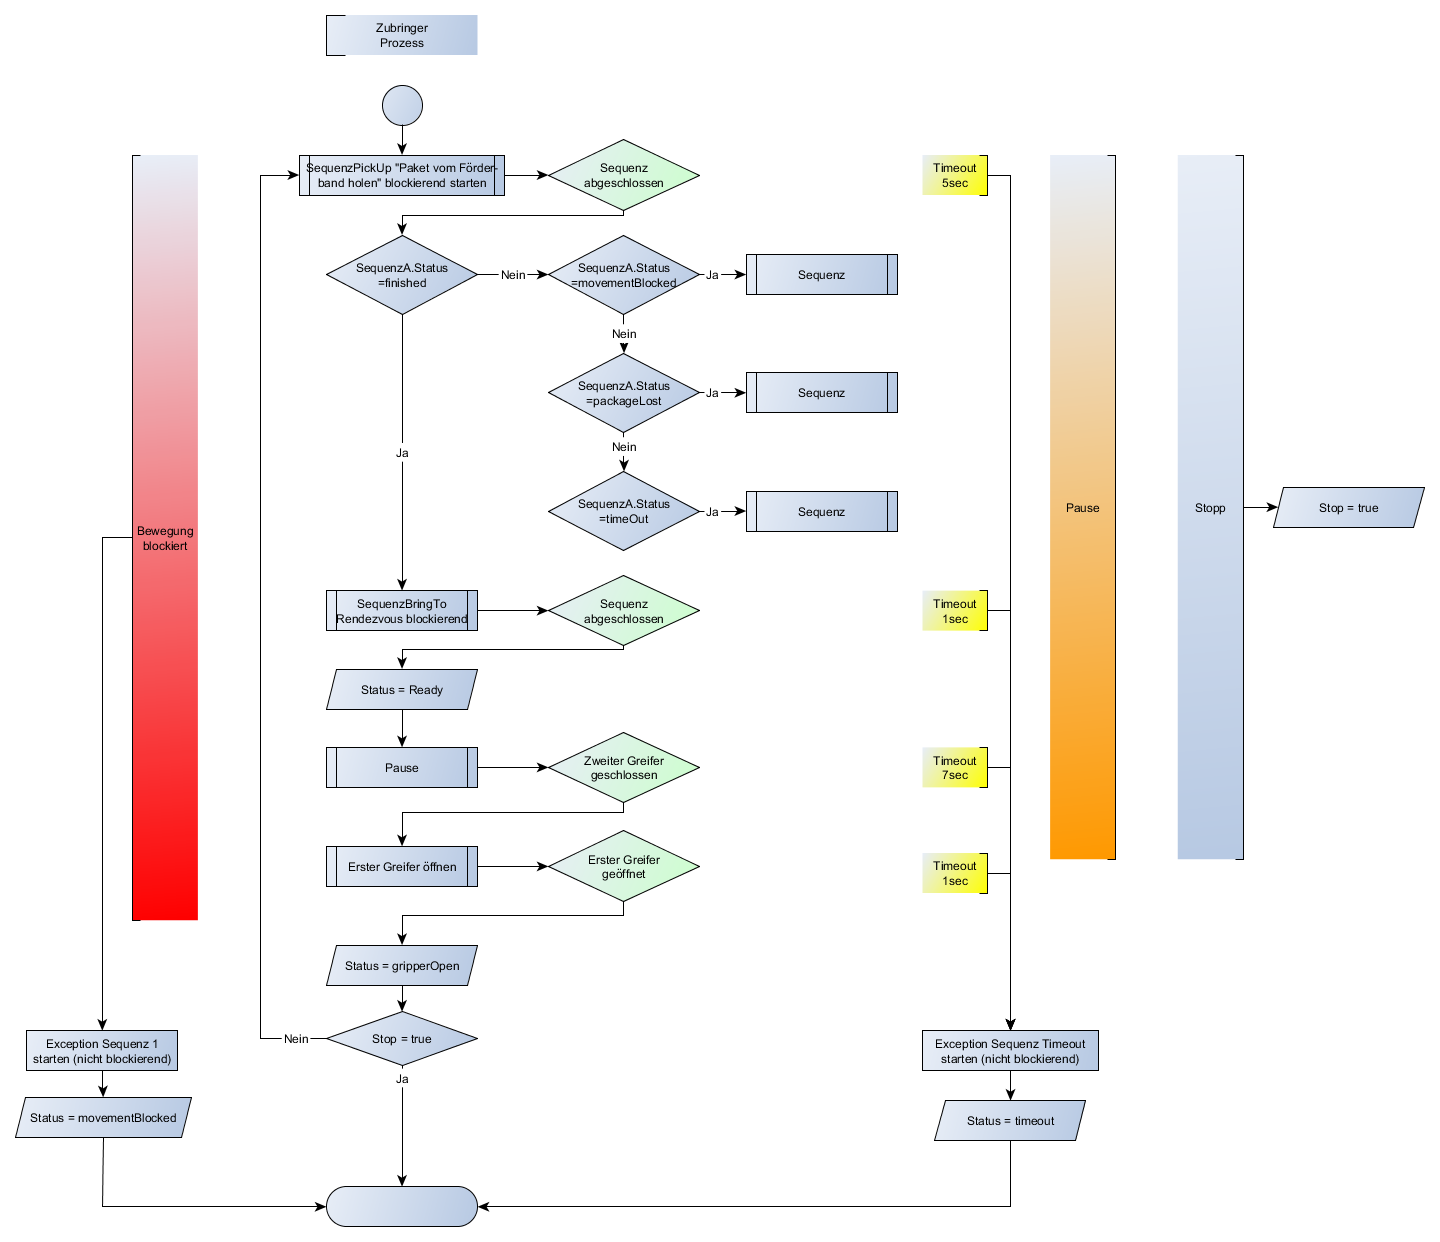
\includegraphics[width=\textwidth]{images/TestCase8Sequence1.png}}
%  \caption{Signalverlauf bei einem prellenden Schalter}
  \label{TestCase8Sequence1Picture}
\end{center}

\begin{center}
  \makebox[\textwidth]{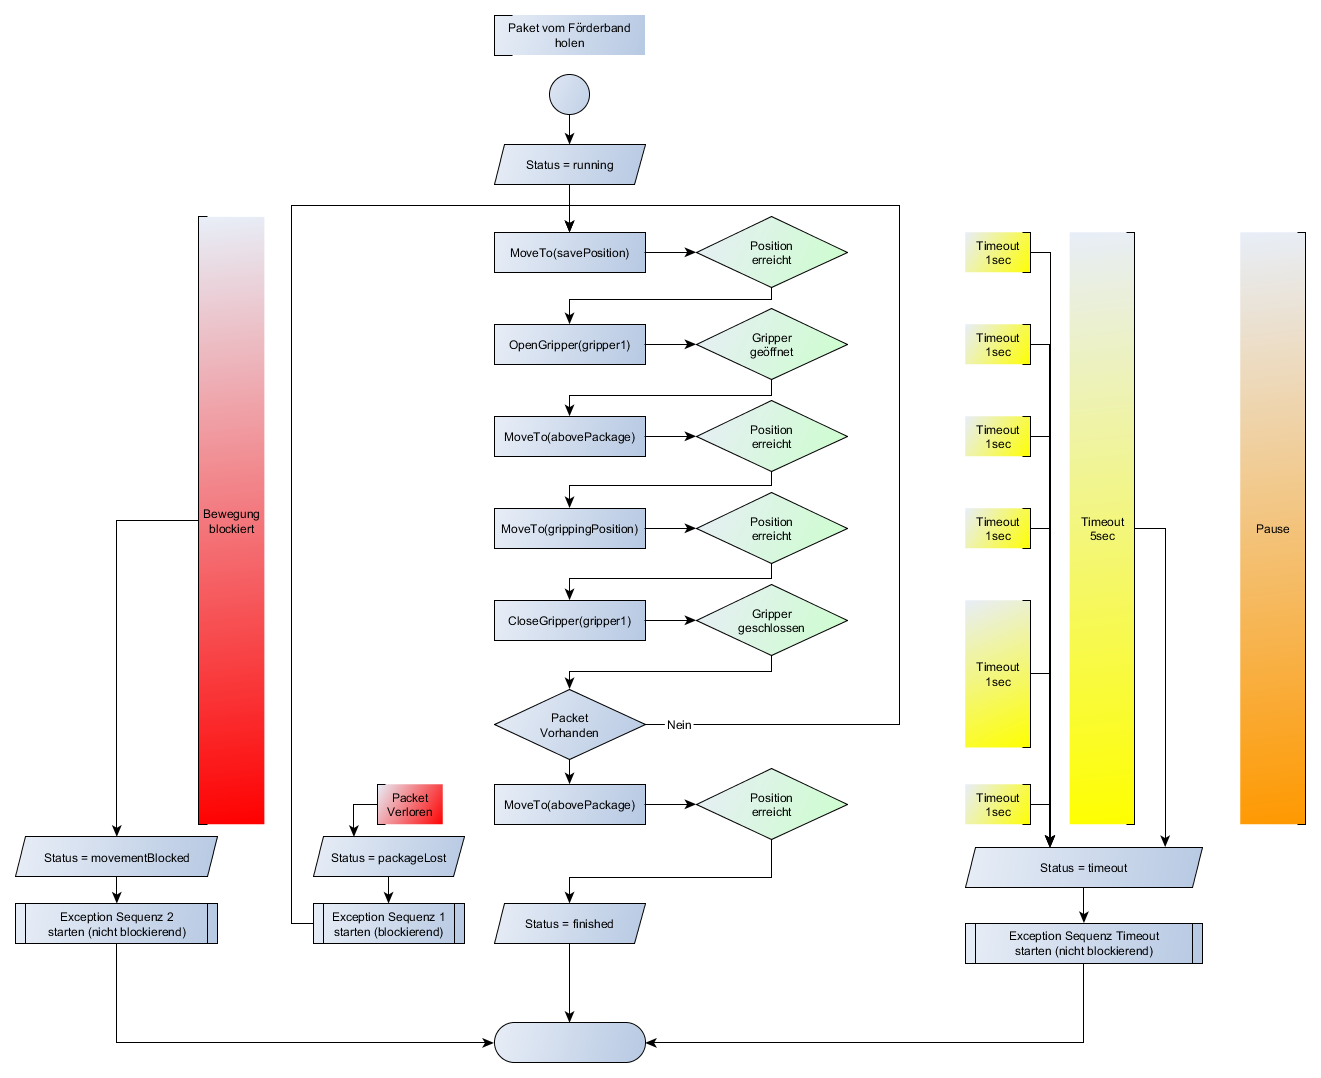
\includegraphics[width=\textwidth]{images/TestCase8Sequence2.png}}
%  \caption{Signalverlauf bei einem prellenden Schalter}
  \label{TestCase8Sequence2Picture}
\end{center}



%\subsection{Skizze Befestigungsbohrungen}\label{sec:anhang_befestigungsbohrungen}
%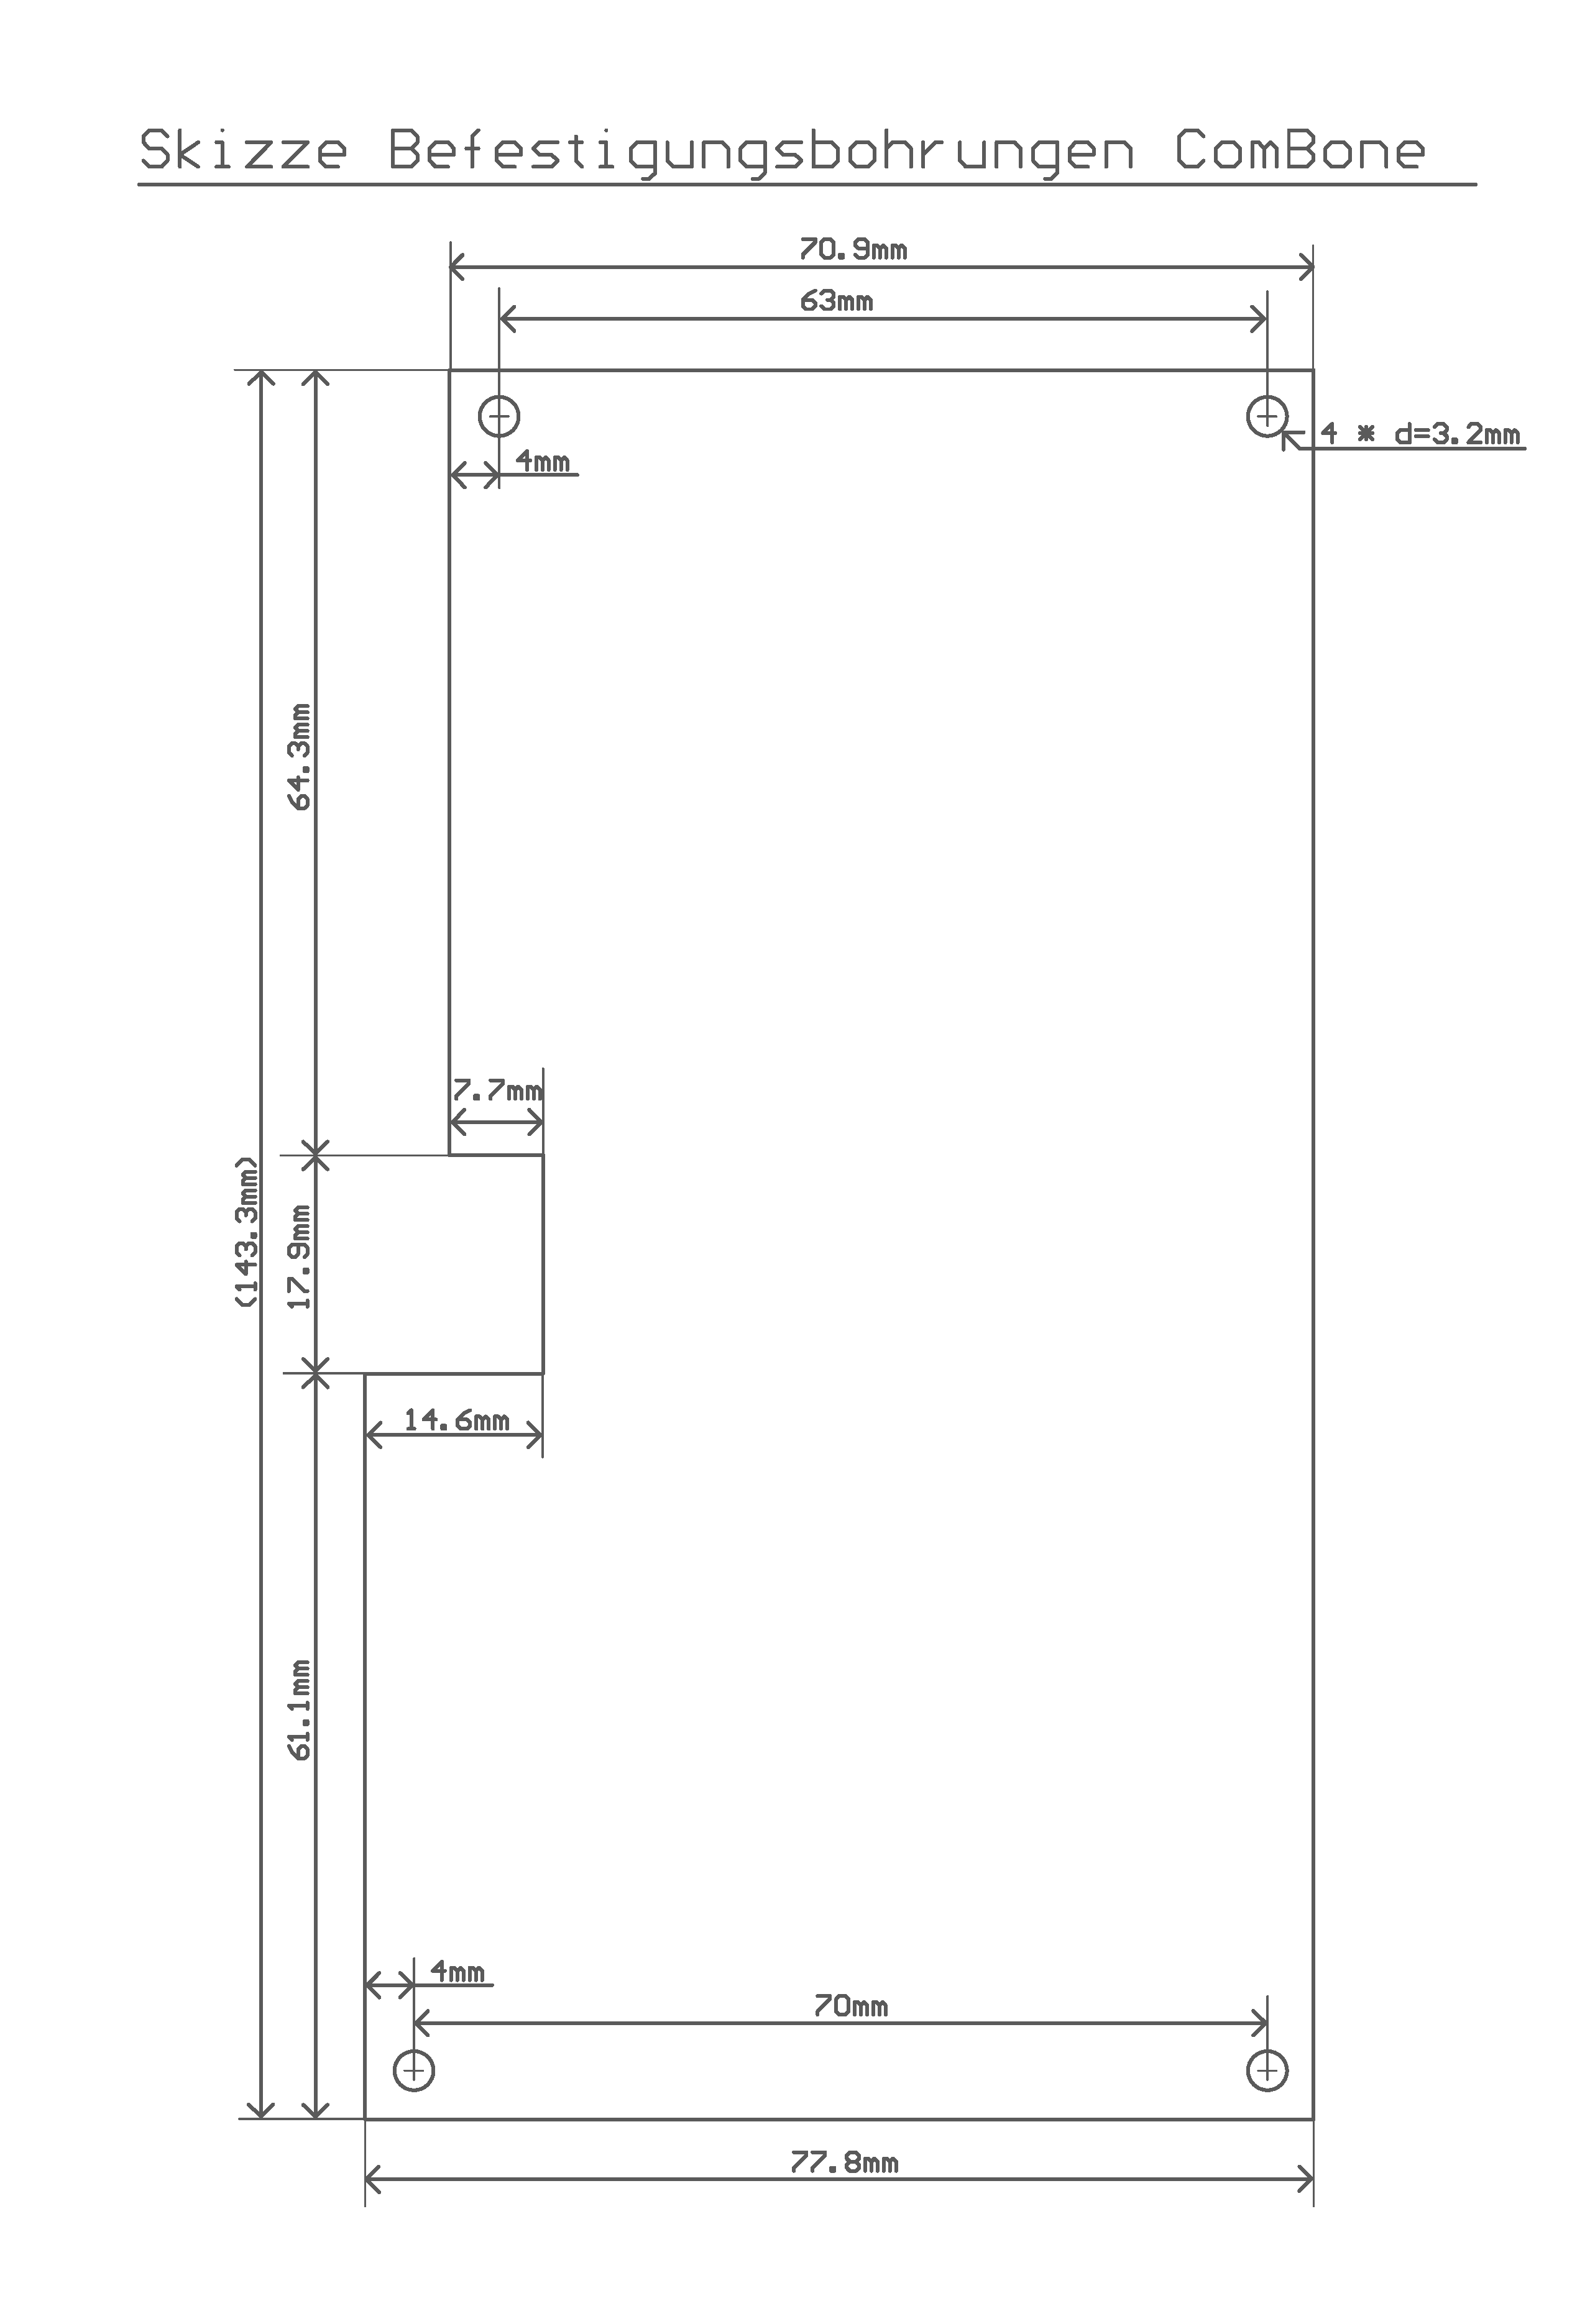
\includepdf[pages=-,pagecommand={\thispagestyle{scrheadings}},angle=0,scale=0.8,frame]{anhang/Elektronik/Skizze_Befestigungsbohrung_ComCape.PDF}




		
		
%
	\end{nosectionintoc}

\end{document}
